\documentclass[]{article}
\usepackage{lmodern}
\usepackage{amssymb,amsmath}
\usepackage{ifxetex,ifluatex}
\usepackage{fixltx2e} % provides \textsubscript
\ifnum 0\ifxetex 1\fi\ifluatex 1\fi=0 % if pdftex
  \usepackage[T1]{fontenc}
  \usepackage[utf8]{inputenc}
\else % if luatex or xelatex
  \ifxetex
    \usepackage{mathspec}
  \else
    \usepackage{fontspec}
  \fi
  \defaultfontfeatures{Ligatures=TeX,Scale=MatchLowercase}
\fi
% use upquote if available, for straight quotes in verbatim environments
\IfFileExists{upquote.sty}{\usepackage{upquote}}{}
% use microtype if available
\IfFileExists{microtype.sty}{%
\usepackage{microtype}
\UseMicrotypeSet[protrusion]{basicmath} % disable protrusion for tt fonts
}{}
\usepackage[margin=1in]{geometry}
\usepackage{hyperref}
\hypersetup{unicode=true,
            pdftitle={STA 303 Assignment 1},
            pdfauthor={Guanchen Zhang},
            pdfborder={0 0 0},
            breaklinks=true}
\urlstyle{same}  % don't use monospace font for urls
\usepackage{graphicx,grffile}
\makeatletter
\def\maxwidth{\ifdim\Gin@nat@width>\linewidth\linewidth\else\Gin@nat@width\fi}
\def\maxheight{\ifdim\Gin@nat@height>\textheight\textheight\else\Gin@nat@height\fi}
\makeatother
% Scale images if necessary, so that they will not overflow the page
% margins by default, and it is still possible to overwrite the defaults
% using explicit options in \includegraphics[width, height, ...]{}
\setkeys{Gin}{width=\maxwidth,height=\maxheight,keepaspectratio}
\IfFileExists{parskip.sty}{%
\usepackage{parskip}
}{% else
\setlength{\parindent}{0pt}
\setlength{\parskip}{6pt plus 2pt minus 1pt}
}
\setlength{\emergencystretch}{3em}  % prevent overfull lines
\providecommand{\tightlist}{%
  \setlength{\itemsep}{0pt}\setlength{\parskip}{0pt}}
\setcounter{secnumdepth}{0}
% Redefines (sub)paragraphs to behave more like sections
\ifx\paragraph\undefined\else
\let\oldparagraph\paragraph
\renewcommand{\paragraph}[1]{\oldparagraph{#1}\mbox{}}
\fi
\ifx\subparagraph\undefined\else
\let\oldsubparagraph\subparagraph
\renewcommand{\subparagraph}[1]{\oldsubparagraph{#1}\mbox{}}
\fi

%%% Use protect on footnotes to avoid problems with footnotes in titles
\let\rmarkdownfootnote\footnote%
\def\footnote{\protect\rmarkdownfootnote}

%%% Change title format to be more compact
\usepackage{titling}

% Create subtitle command for use in maketitle
\newcommand{\subtitle}[1]{
  \posttitle{
    \begin{center}\large#1\end{center}
    }
}

\setlength{\droptitle}{-2em}

  \title{STA 303 Assignment 1}
    \pretitle{\vspace{\droptitle}\centering\huge}
  \posttitle{\par}
    \author{Guanchen Zhang}
    \preauthor{\centering\large\emph}
  \postauthor{\par}
      \predate{\centering\large\emph}
  \postdate{\par}
    \date{July 14, 2018}

\usepackage{amsmath}
\usepackage{commath}
\usepackage{geometry}
\usepackage{setspace}
\onespacing
\geometry{top=1in}
\newcommand{\ed}{\overset{d}{=}}
\newcommand{\cp}{\overset{p}{\rightarrow}}
\newcommand{\cd}{\overset{d}{\rightarrow}}
\renewcommand{\baselinestretch}{1.5}
\newcommand{\mb}[1]{\ensuremath{\boldsymbol{\mathbf{#1}}}}
\usepackage{sectsty} \sectionfont{\centering \emph}
\usepackage{xcolor}
\usepackage{fetamont}
\newcommand*\eiadfamily{\fontencoding{OT1}\fontfamily{times}\selectfont}
\newcommand{\mytitle}{\eiadfamily}
\newcommand{\myauthor}{\ffmfamily \textcolor{blue}}
\pretitle{\vspace{\droptitle}\centering\eiadfamily\emph}
\usepackage{multicol}

\begin{document}
\maketitle

\fontsize{12}{12} \selectfont

\subsection{Gauge Calibration}\label{gauge-calibration}

To monitor the water supply,people wants to analysize the snow-pack
profile because show absorb the water up to a certain point, after which
the water floods away. The snow gauge is used to determine a depth
profile of snow density but does not directly measure snow density. The
experimental data were acquired by varying density and measuring the
gain. In the experiment, the polyethylene blocks are used to simulate
snow whose density was recorded in dataset. The gauge measurement is
called ``gain''.

In the context of the problem, a statistical model is necessay and ther
is no alternative way. In general, linear regression has following
assumptions: Linear relationship, Multivariate normality, No
multicollinearity (no need in this case), No auto-correlation (no need
in this case), Homoscedasticity. A simple linear regression model called
fit1 was built to estimate mean density at a given gain. From the
diagnostic plots of the fit1 model, there is a distinctive curvilinear
pattern in the residual vs.~fitted plot (figure 1.2). This could mean
that we may get a better model is we try a model with a quadratic term
included. The assumption of equal variance does not hold under the model
of fit1.

When the variance is found to be nonconstant, we can consider to use
transformation to stabilize variance. Also because the relationship
between the response and the design variable is not linear, it is
possible that a transormataion can put the relationship into a linear
form. According to the boxcox function in R, a log transformation is
recommended since the lamda is 0 which is acceptable for the log
transformation. The resulting scatter plot has points forming a nearly
perfect straightline, indicating an almost linear relationship. All
assumptions for linear regression hold under the model of fit2.

Since the scatter plot is curved, a polynomial model may be appropriate.
However, the physical model for the relationship between gain and
density suggests proceeding with the log transformation.

Then we can conclude that to estimate mean density of snow pack at given
gain we can use the model depicted as fit2 by taking log to ``gain''.

\subsection{Appendix}\label{appendix}

We first need to coerce other objects to a data frame and glimpse at the
data frame (table 1.1). There are 90 observations and 2 variables which
are density and gain.

Then, a scatter plot of density by gain was plotted (figure 1.1), which
indicates there is a curvilinear relationship instead of linear
relationship where the density decrease exponentially when the gain
increase.

\subsubsection{Table 1.1 Glimpse}\label{table-1.1-glimpse}

\begin{verbatim}
## Observations: 90
## Variables: 2
## $ density <dbl> 0.686, 0.686, 0.686, 0.686, 0.686, 0.686, 0.686, 0.686...
## $ gain    <dbl> 17.6, 17.3, 16.9, 16.2, 17.1, 18.5, 18.7, 17.4, 18.6, ...
\end{verbatim}

\includegraphics{assignment_1_files/figure-latex/unnamed-chunk-2-1.pdf}
The assumption of normal errors is needed and can be checked by QQ plot
(figure 1.3). In the normal QQ plot (figure 1.3) produces points close
to a straight line so the data are said to be consistent with that from
a normal distribution. Another assumption is that the errors have
constant variance. In the residual vs.~fitted plot (figure 1.2), the
residuals are not spread equally around 0, indicating the assumption of
equal variance is violated.

\subsubsection{Table 1.2 ANOVA of fit1}\label{table-1.2-anova-of-fit1}

\begin{verbatim}
## Analysis of Variance Table
## 
## Response: density
##           Df Sum Sq Mean Sq F value    Pr(>F)    
## gain       1 3.7169  3.7169  389.48 < 2.2e-16 ***
## Residuals 88 0.8398  0.0095                      
## ---
## Signif. codes:  0 '***' 0.001 '**' 0.01 '*' 0.05 '.' 0.1 ' ' 1
\end{verbatim}

\includegraphics{assignment_1_files/figure-latex/unnamed-chunk-3-1.pdf}
\includegraphics{assignment_1_files/figure-latex/unnamed-chunk-3-2.pdf}

In the residual vs.~fitted plot (figure 1.6), the residuals are spread
equally around 0, indicating the assumption of equal variance is hold
and the curvilinear pattern is not such obvious as the original model.
Meanwhile, the assumption of normal errors is improved in the QQ plot
(figure 1.5). Moreover, because the smaller the residual sum of squares,
the better your model fits your data, comparing ANOVA of fit1 (table
1.2) with that of fit2 (table 1.3), the residual sum of squres of the
fit2 is much smaller than that of fit1 and more closer to 0.

\subsubsection{Table 1.3 ANOVA of fit2}\label{table-1.3-anova-of-fit2}

\begin{verbatim}
## Analysis of Variance Table
## 
## Response: density
##              Df Sum Sq Mean Sq F value    Pr(>F)    
## I(log(gain))  1 4.5376  4.5376   20956 < 2.2e-16 ***
## Residuals    88 0.0191  0.0002                      
## ---
## Signif. codes:  0 '***' 0.001 '**' 0.01 '*' 0.05 '.' 0.1 ' ' 1
\end{verbatim}

\includegraphics{assignment_1_files/figure-latex/unnamed-chunk-4-1.pdf}

\begin{verbatim}
## [1] 0.02020202
\end{verbatim}

\includegraphics{assignment_1_files/figure-latex/unnamed-chunk-4-2.pdf}
\includegraphics{assignment_1_files/figure-latex/unnamed-chunk-4-3.pdf}
\includegraphics{assignment_1_files/figure-latex/unnamed-chunk-4-4.pdf}

\subsection{Dugeness crabs}\label{dugeness-crabs}

Dugeness crabs are fished extensively and fisihing female crabs is a
possible means of controlling hte fluctuation in yearly catches of
crabs. To determine size restrictions for female crabs, we are trying to
estimate mean carapace size for crabs who have recently molted, for
those who have not, and whether the difference is significant. The shell
width was recorded as ``size'' in the dataset and information on whether
the crab had molted in the most recent molting season or not was
recorded as dummy variable called ``shell''. According to the background
reading, ``shell'' is 0 means the crab has a fouled shell indicating it
had molted in the most recent molting season, whereas, 1 means the crab
has a clean shell, indicating it had not molted in the most recent
molting season.

A box plot (Figure 2.1) is drawn as well which enable us to study the
distributional characteristics of the group of the variable and provide
some indication of the data's symmetry and skewness. Unlike other
methods of data display, boxplots show outliers. By using a boxplot for
each categorical variable side-by-side, it is easy to compare data set.

Regarding the problem of the crab growth, ANOVA is used to assess the
relationship between a continuous and categorical variable, unlike the
linear regression model used to solve the problem of gauge calibration
where both the dependent variable and the independent variable are
continuous.

Then we can conclude that estimated mean carapace size for crabs who
have recently molted is 142cm, for those who have not is 149cm, and
there is significant evidence that whether the female crab had molted in
the most recent molting season or not impact on the width of the female
crab.

\subsection{Appendix}\label{appendix-1}

In general, the shape of the box are different between fouled shell and
clean shell crab. Comparing the box for clean shell, the box for fouled
shell is much shorter, suggesting that size of fouled shell carbs have a
high level of agreement with each other, meanwhile, it is much higher,
suggesting a difference between groups. Regarding the boxplot for clean
shell carbs, the box are uneven in size, showing that many carbs have
similar sizes at certain parts of the scale, but in other parts of the
parts of scale sizes of clean carbs vary much. Outliers are very
noticable for the carbs with fouled shell. \#\#\# Table 2.1 Glimpse

\begin{verbatim}
## Observations: 362
## Variables: 2
## $ size  <dbl> 116.8, 117.1, 118.4, 119.6, 120.1, 120.4, 120.6, 122.6, ...
## $ shell <chr> "1", "1", "1", "1", "1", "1", "1", "1", "1", "1", "1", "...
\end{verbatim}

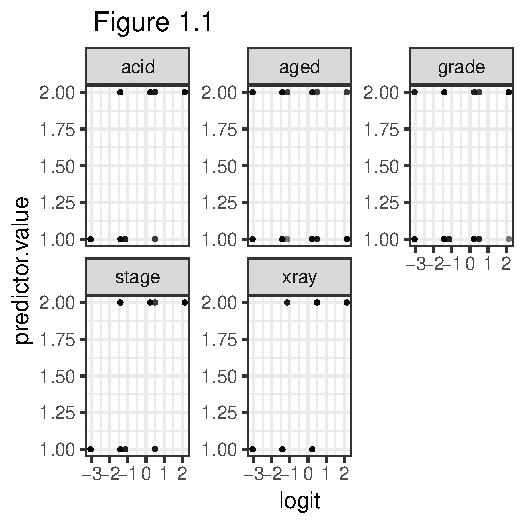
\includegraphics{assignment_1_files/figure-latex/unnamed-chunk-6-1.pdf}

\subsubsection{Table 2.2 Grand
statistics}\label{table-2.2-grand-statistics}

\begin{verbatim}
## # A tibble: 1 x 2
##   grand_mean grand_sd
##        <dbl>    <dbl>
## 1       145.     11.8
\end{verbatim}

\subsubsection{Table 2.3 Group
statistics}\label{table-2.3-group-statistics}

\begin{verbatim}
## 
## Call:
## lm(formula = size ~ shell, data = crabs_t)
## 
## Residuals:
##     Min      1Q  Median      3Q     Max 
## -53.710  -5.986  -0.260   7.789  22.987 
## 
## Coefficients:
##             Estimate Std. Error t value Pr(>|t|)    
## (Intercept) 149.1099     0.8938 166.823  < 2e-16 ***
## shell1       -6.9965     1.1995  -5.833 1.21e-08 ***
## ---
## Signif. codes:  0 '***' 0.001 '**' 0.01 '*' 0.05 '.' 0.1 ' ' 1
## 
## Residual standard error: 11.34 on 360 degrees of freedom
## Multiple R-squared:  0.08634,    Adjusted R-squared:  0.08381 
## F-statistic: 34.02 on 1 and 360 DF,  p-value: 1.215e-08
\end{verbatim}

\begin{verbatim}
## # A tibble: 2 x 5
##   shell count median  mean    sd
##   <chr> <int>  <dbl> <dbl> <dbl>
## 1 0       161   151.  149.  11.3
## 2 1       201   141.  142.  11.4
\end{verbatim}

In the ANOVA table(table 2.4), as the p-value is less than the
significance level 0.05, we can conclude that there are significant
differences between the group of fouled shell carbs and the group of
clean shell carbs. Since there are only 2 groups, it is not necessary to
perform multiple pairwise-comparison, to determine if the mean
difference between specific pairs of group are statistically
significant.

The ANOVA test assumes that, the data are normally distributed and the
variance across groups are homogeneous. From the output (table 2.5) we
can see that the p-value is not less than the significance level of
0.05. This means that there is no evidence to suggest that the variance
across groups is statistically significantly different. Therefore, the
assumption of homogeneity of variances in the different treatment groups
holds. Anova assumes that the data in each group are distributed
normally. This assumption is equivalent saying that the residuals of the
best-fitting model are distributed normally. In the normal QQ plot
(Figure 2.2), as almost all the points fall approximately along this
reference line, the assumption holds.

\subsubsection{Table 2.4 ANOVA table}\label{table-2.4-anova-table}

\begin{verbatim}
##              Df Sum Sq Mean Sq F value   Pr(>F)    
## shell         1   4376    4376   34.02 1.21e-08 ***
## Residuals   360  46305     129                     
## ---
## Signif. codes:  0 '***' 0.001 '**' 0.01 '*' 0.05 '.' 0.1 ' ' 1
\end{verbatim}

\includegraphics{assignment_1_files/figure-latex/unnamed-chunk-10-1.pdf}

\subsubsection{Table 2.5 Equal variance
test}\label{table-2.5-equal-variance-test}

\begin{verbatim}
## 
##  Bartlett test of homogeneity of variances
## 
## data:  size by shell
## Bartlett's K-squared = 0.022512, df = 1, p-value = 0.8807
\end{verbatim}


\end{document}
